\documentclass[11pt]{article}
\usepackage[utf8x]{inputenc}
\usepackage[T1]{fontenc}
\usepackage[spanish]{babel}
\usepackage{caption}
\usepackage{fixltx2e}
\usepackage{graphicx}
\usepackage{longtable}
\usepackage{float}
\usepackage{wrapfig}
\usepackage{rotating}
\usepackage[normalem]{ulem}
\usepackage{amsmath}
\usepackage{textcomp}
\usepackage{marvosym}
\usepackage{wasysym}
\usepackage{amssymb}
\usepackage{hyperref}
\tolerance=1000
\author{Daniel Fernández Pérez\\Miguel García-Mauriño Taboada}
\date{\today}
\title{Reconocimiento de iconos}
\hypersetup{
  pdfencoding=auto,
  pdfkeywords={},
  pdfsubject={},
  hidelinks=true,
  pdfcreator={Emacs 25.1.1 (Org mode 8.2.10)}}
\begin{document}
\begin{titlepage}
  \clearpage
  \maketitle
  \thispagestyle{empty}
\end{titlepage}
\pagebreak
\tableofcontents
\pagebreak
\section{Introducción}
Los iconos de señalización sirven para que las personas localicen determinados puntos de interés en un entorno. Esto podría entenderse desde un punto de vista informático como ``añadir semántica a un mapa''. Así, también es beneficioso para un robot ser capaz de reconocer iconos, puesto que permite tanto añadir semántica a un mapa como localizarse dentro de dicho mapa si la localización por otros medios no es posible (por ejemplo, el GPS no funciona correctamente en interiores).

El objetivo de este trabajo es implementar y comparar el rendimiento de distintos clasficadores para el problema del reconocimiento de iconos. Para ello, partimos de un universo de trabajo con cuatro iconos.

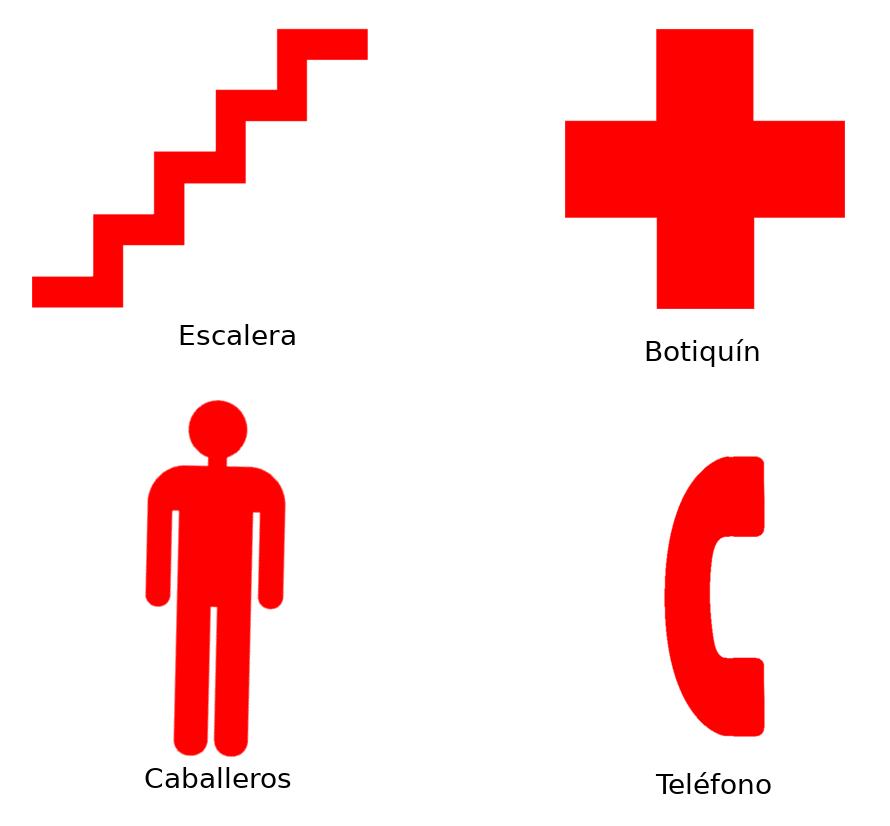
\includegraphics[width=.9\linewidth]{rsc/universo.png}
\captionof{figure}{Iconos del universo de trabajo}

Los clasificadores que vamos a evaluar son de tipo \textit{K vecinos más próximos} con $K=1$, uno de ellos con la distancia euclídea y el otro con la distancia de Mahalanobis. Los entrenaremos en un espacio de las siete dimensiones correspondientes a los siete momentos invariantes de Hu de cada uno de los iconos.

\section{Creación del \textit{dataset} de entrenamiento}

Para crear el \textit{dataset} de entrenamiento necesitábamos al menos cien datos independientes de cada uno de los iconos (es decir, que no estuvieran deducidos unos de otros). Para ello era necesario tomar el mismo número de fotografías. Como esto requería mucho trabajo, decidimos grabar un vídeo por cada icono y tomar cien de sus fotogramas. En el vídeo cambiábamos la posición relativa entre el icono y la cámara con el fin de que los datos recogidos fueran lo más representativos posible. Una vez extraidos los datos de cada icono, guardamos el \textit{dataset} en un fichero de texto para que no fuera necesario procesar los vídeos cada vez que realizábamos alguna prueba.

\subsection{Extracción de los momentos de Hu de un icono}

Para extraer los momentos de Hu del icono es necesario primero diferenciar qué píxeles de la imagen son de icono y cuáles son de otra cosa (fondo, línea, etc). Para resolver este problema recurrimos a una segmentación basada en colores que utiliza un clasificador basado en la distancia euclídea. Tras la ejecución de dicha segmentación, obtenemos una imagen binaria que muestra tan solo el icono. A continuación, podemos utilizar las funciones de la biblioteca de opencv de python para encontrar el contorno y los momentos de Hu correspondientes al icono.

\section{Creación y validación de los reconocedores}

Para la implementación de los reconocedores hemos utilizado la biblioteca de scikit-learn de python, que implementa los dos reconocedores sobre los que trabajamos de forma eficiente y simplifica su uso al usuario. Después de esta implementación tan simple, pasamos a la validación.

La validación de los clasificadores se realiza mediante el método \textit{leaving one out}: Para cada uno de los vectores $v$ de datos en el \textit{dataset}, se entrena el clasificador con los vectores de $dataset \ v$, es decir, con todo el dataset excluyendo el vector $v$. A continuación, se ejecuta el clasificador entrenado sobre $v$ y se toma nota de si la clasificación ha sido correcta. Finalmente, tras el bucle, se calcula el porcentaje de aciertos del clasificador.

\section{Reconocimiento de inconos en un vídeo}

Para probarlo en un caso más similar al real, hemos grabado un recorrido con el robot en el que aparecen los iconos del universo de trabajo. El reconocimiento de iconos se ha realizado de la siguiente manera:
\\
Para cada fotograma:
\begin{enumerate}
\item Segmentar la imagen para obtener sólo los píxeles que pertenecen a un icono.
\item Quedarnos con el mayor contorno de la imagen, para el caso de que la segmentación no haya funcionado a la perfección.
\item Si el contorno está en el borde, pasar al siguiente fotograma y volver a empezar. Si no, continuar.
\item Sobre el contorno obtenido, calcular los momentos de Hu del icono.
\item Ejecutar el clasificador sobre los momentos de Hu obtenidos para obtener la etiqueta del icono.
\item \textit{(Solo para generar video:)} Dibujar el contorno sobre el icono e imprimir la etiqueta en el fotograma del vídeo
\end{enumerate}

\section{Resultados}
\subsection{Rendimiento de los reconocedores}
\begin{table}[ht]

  \begin{tabular}{|l|l|}
    \hline
    Clasificador & Rendimiento\\
    \hline\hline
    1-NN Euclídeo  & 384 correctos de 415 (92,53\% de aciertos)\\
    \hline
    1-NN Mahalanobis  & 415 correctos de 415 (92,53\% de aciertos)\\\hline

  \end{tabular}
  \caption{Comparativa de rendimiento de los reconocedores}\label{table-rendimiento}

\end{table}
Como se puede ver en la tabla~\ref{table-rendimiento}, el reconocedor basado en la distancia de Mahalanobis funciona perfectamente, mientras que el otro, aunque tiene una tasa de aciertos relativamente elevada, comete algunos fallos, por lo que es evidente que la elección correcta para la clasificación del vídeo del recorrido es el que utiliza la distancia de Mahalanobis.

\subsection{Reconocimiento de iconos en un recorrido}
Como se puede ver en el video adjunto, el reconocedor funciona de forma correcta y estable para los cuatro iconos del universo de trabajo.
\section{Conclusiones}
La principal conclusión que sacamos tras este trabajo es que la distancia de Mahalanobis funciona mucho mejor que la distancia euclídea, al menos para el caso de reconocimiento de iconos. Además, notamos la importancia de tener un buen dataset de entrenamiento a la hora de trabajar con casos reales, así como de disponer de una buena forma de describir los objetos a reconocer. Para este caso, ``buena'' significa que si dos objetos se parecen mucho o son el mismo, entonces la descripción debe dar valores similares, mientras que si los objetos son diferentes, debe devolver valores suficientemente alejados uno de otro para diferenciarlos. En el caso del reconocimiento de iconos, parece que los momentos de Hu son idóneos como descripción.
\end{document}
